\documentclass[tikz, border=10pt]{standalone}
\usepackage{tikz}
\usetikzlibrary{shapes.geometric, arrows} 

% defining tikz shapes
\tikzstyle{startstop} = [rectangle, minimum width=3cm, minimum height=1cm,inner sep=8pt,text centered, draw=black, fill=blue!30]
\tikzstyle{process} = [rectangle, minimum width=3cm, minimum height=1cm, inner sep=8pt,  text centered, draw=black, fill=orange!30]
\tikzstyle{io} = [rectangle, inner sep=8pt, text centered, draw=black, fill=gray!15]
\tikzstyle{arrow} = [thick,->,>=stealth]

\begin{document}

%%%%%%%%%%%%%%%
% Pipeline workflow figure
%%%%%%%%%%%%%%%

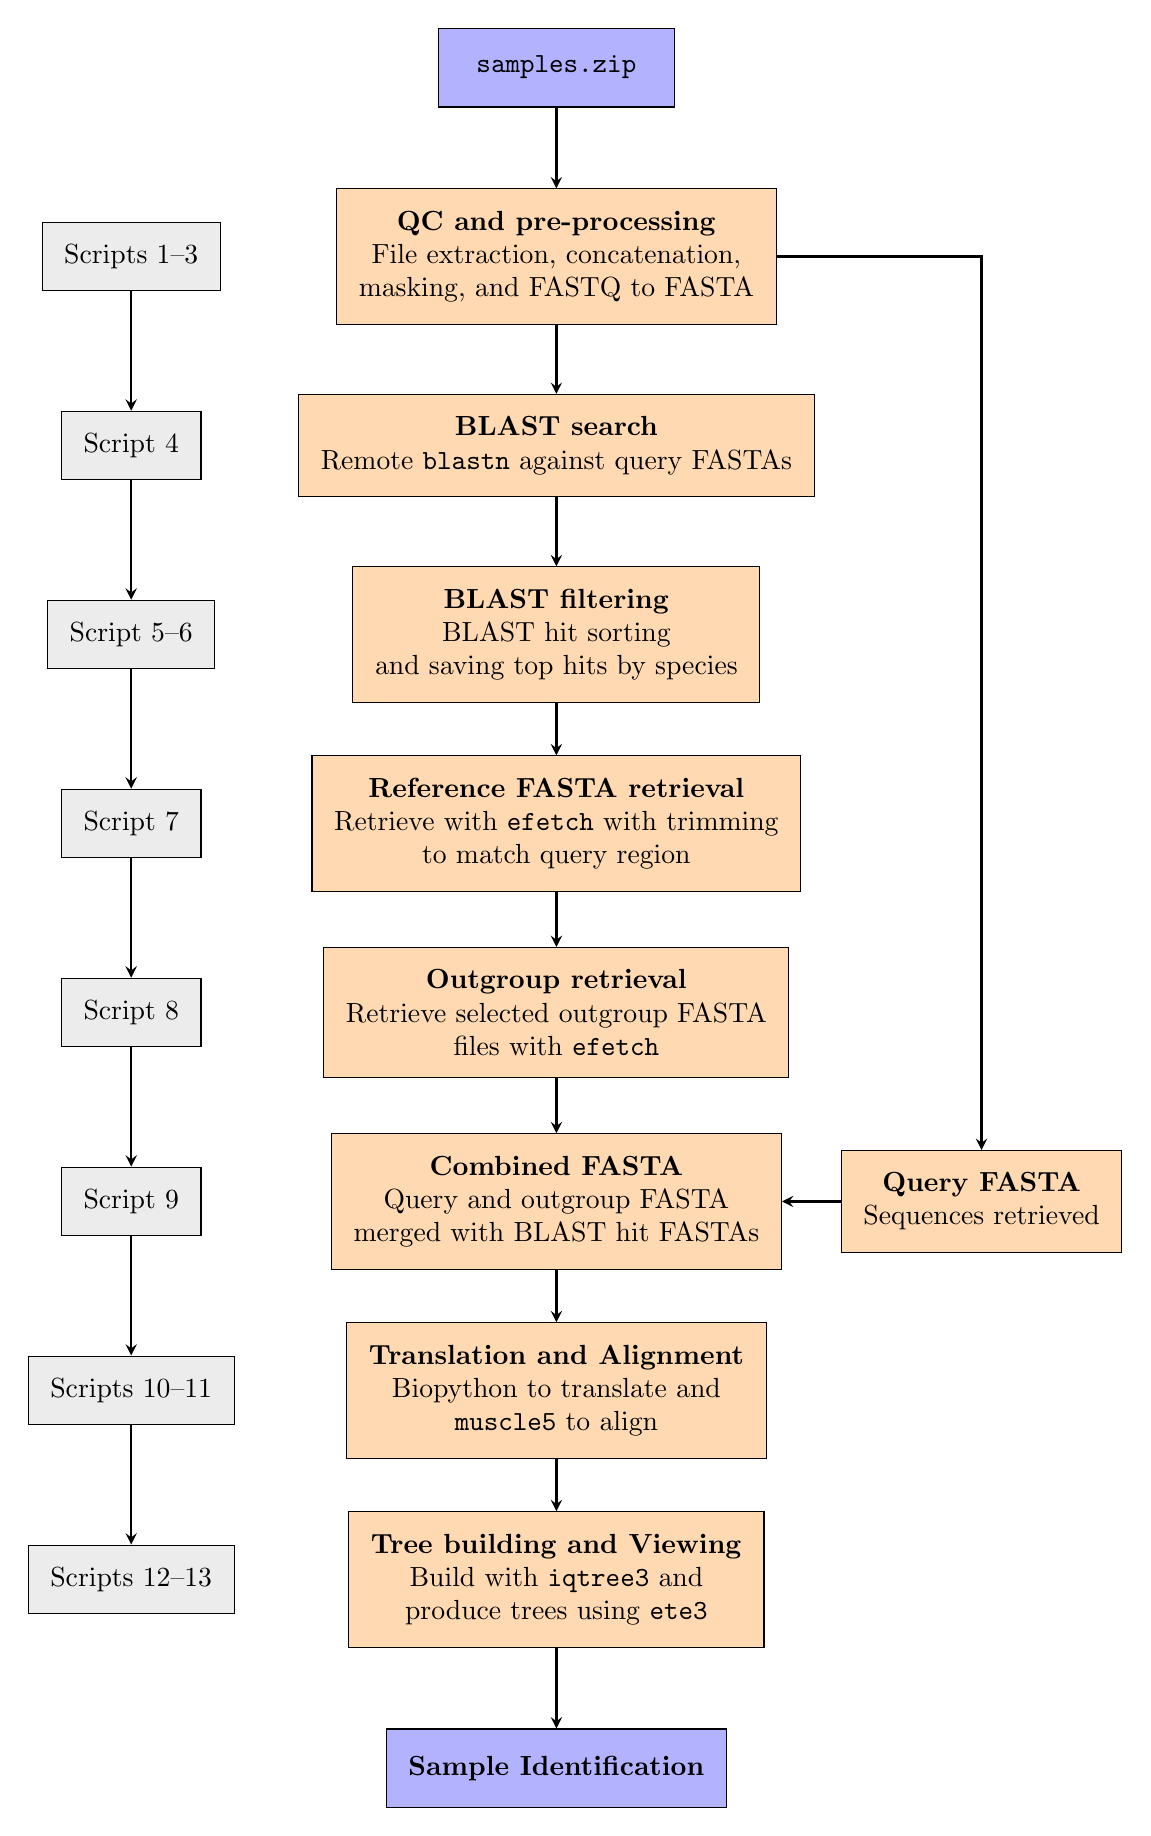
\begin{tikzpicture}[node distance=2.4cm]
				\node (start) [startstop] {{\texttt{samples.zip}}};
				\node (pro2) [process, below of=start, align=center] {\textbf{QC and pre-processing}\\File extraction, concatenation, \\masking, and FASTQ to FASTA};
				\node (pro3) [process, below of=pro2, align=center] {\textbf{BLAST search}\\Remote \texttt{blastn} against query FASTAs};
				\node (pro4) [process, below of=pro3, align=center] {\textbf{BLAST filtering}\\ BLAST hit sorting \\and saving top hits by species};\textsc{}
				\node (pro5) [process, below of=pro4, align=center] {\textbf{Reference FASTA retrieval}\\Retrieve with \texttt{efetch} with trimming \\to match query region};
				\node (pro6) [process, below of=pro5, align=center] {\textbf{Outgroup retrieval}\\Retrieve selected outgroup FASTA \\files with \texttt{efetch}};
				\node (pro7a) [process, below of=pro6, align=center] {\textbf{Combined FASTA}\\Query and outgroup FASTA \\merged with BLAST hit FASTAs};
				\node (pro7b) [process, right of=pro7a, align=center] at ([xshift=3cm]pro7a) {\textbf{Query FASTA}\\ Sequences retrieved};
				\node (pro8) [process, below of=pro7a, align=center] {\textbf{Translation and Alignment}\\Biopython to translate and \\\texttt{muscle5} to align};
				\node (pro9) [process, below of=pro8, align=center] {\textbf{Tree building and Viewing}\\Build with \texttt{iqtree3} and \\produce trees using \texttt{ete3}};
				\node (stop) [startstop, below of=pro9, align=center] {\textbf{Sample Identification}};
				
				\node (scr1) [io, left of=pro2, align=center] at ([xshift=-3cm]pro2) {Scripts 1--3};
				\node (scr2) [io, left of=pro3, align=center] at ([xshift=-3cm]pro3) {Script 4};
				\node (scr3) [io, left of=pro4, align=center] at ([xshift=-3cm]pro4) {Script 5--6};
				\node (scr4) [io, left of=pro5, align=center] at ([xshift=-3cm]pro5) {Script 7};
				\node (scr5) [io, left of=pro6, align=center] at ([xshift=-3cm]pro6) {Script 8};
				\node (scr6) [io, left of=pro7a, align=center] at ([xshift=-3cm]pro7a) {Script 9};
				\node (scr7) [io, left of=pro8, align=center] at ([xshift=-3cm]pro8) {Scripts 10--11};
				\node (scr8) [io, left of=pro9, align=center] at ([xshift=-3cm]pro9) {Scripts 12--13};
				
				\draw [arrow] (start) -- (pro2);
				\draw [arrow] (pro2) -- (pro3);
				\draw [arrow] (pro3) -- (pro4);
				\draw [arrow] (pro4) -- (pro5);
				\draw [arrow] (pro5) -- (pro6);
				\draw [arrow] (pro6) -- (pro7a);
				\draw [arrow] (pro7b) -- (pro7a);
				\draw [arrow] (pro7a) -- (pro8);
				\draw [arrow] (pro8) -- (pro9);
				\draw [arrow] (pro9) -- (stop);
				\draw [arrow] (pro2) -| (pro7b);
				
				\draw [arrow] (scr1) -- (scr2);
				\draw [arrow] (scr2) -- (scr3);
				\draw [arrow] (scr3) -- (scr4);
				\draw [arrow] (scr4) -- (scr5);
				\draw [arrow] (scr5) -- (scr6);
				\draw [arrow] (scr6) -- (scr7);
				\draw [arrow] (scr7) -- (scr8);
				
\end{tikzpicture}


\end{document}